\chapter{Organización temporal}
\label{chap:planificación}

La planificación general del proyecto siguiendo un modelo SCRUM, empleando para ello el panel de tareas Trello; un gestor de proyectos que permite aplicar una metodología de desarrollo ágil.\\

El panel se encuentra accesible en el siguiente enlace: \url{https://trello.com/b/SpIbFI7k/robotui}.

\begin{figure}[H]
\hspace*{-.2in}{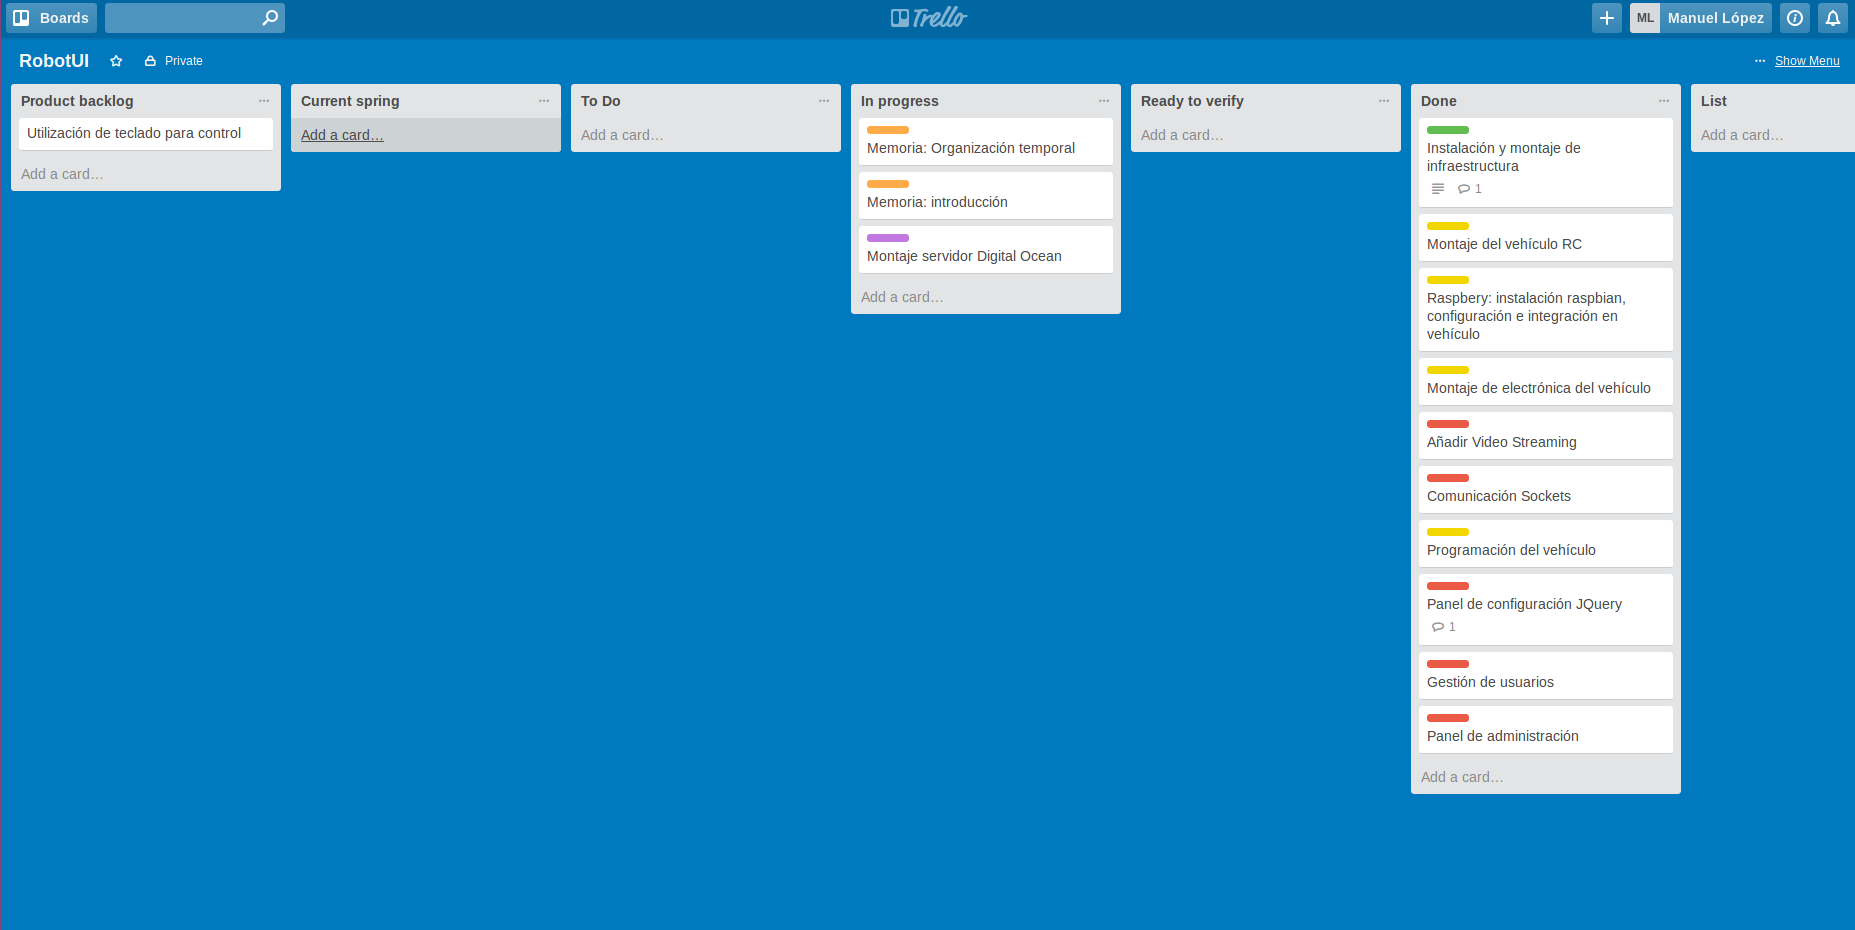
\includegraphics[scale=0.25]{imagenes/panel-trello.png}}
\caption{Panel de actividades - Trello}
\end{figure}


Cabe destacar que para el desarrollo de RobotUI ha sido necesario emplear varias herramientas, utilidades y bibliotecas. Algunas de ellas ya habían sido utilizadas en ciertas ocasiones, bien sea en el ámbito estudiantil o profesional. 
Sin embargo, otras han requerido un periodo de formación previo, en el que se han adquirido los conocimientos necesarios para poder desarrollar el presente proyecto.\\

La mayor parte del proceso de investigación fue dedicado al estudio de las diferentes tecnologías existentes para la programación web en tiempo real. Todo ello ha implicado un esfuerzo bastante considerable en el uso, 
aprendizaje e investigación de las diferentes tecnologías existentes y comprobar su potencial.\\

Una vez determinadas las diferentes herramientas a utilizar se comenzó con la implementación de la aplicación, siendo seleccionada como herramienta principal el framework Sails.js. Un framework MVC en 
tiempo real para Node.js, el cual está muy enfocado al propósito de este proyecto.\\

Finalmente, tras la necesidad de probar la aplicación en un entorno real, se optó por elaborar un robot de pruebas, un pequeño vehículo elaborado con una Raspberry Pi con la finalidad de probar, testear y hacer 
demostraciones de la aplicación.

La figura \ref{gantt:tareas01} y \ref{gantt:tareas02} muestran una visión de las diferentes tareas desarrolladas para la elaboración del proyecto junto con la descomposición de cada una de ellas:\\

\begin{figure}
  \begin{center}
    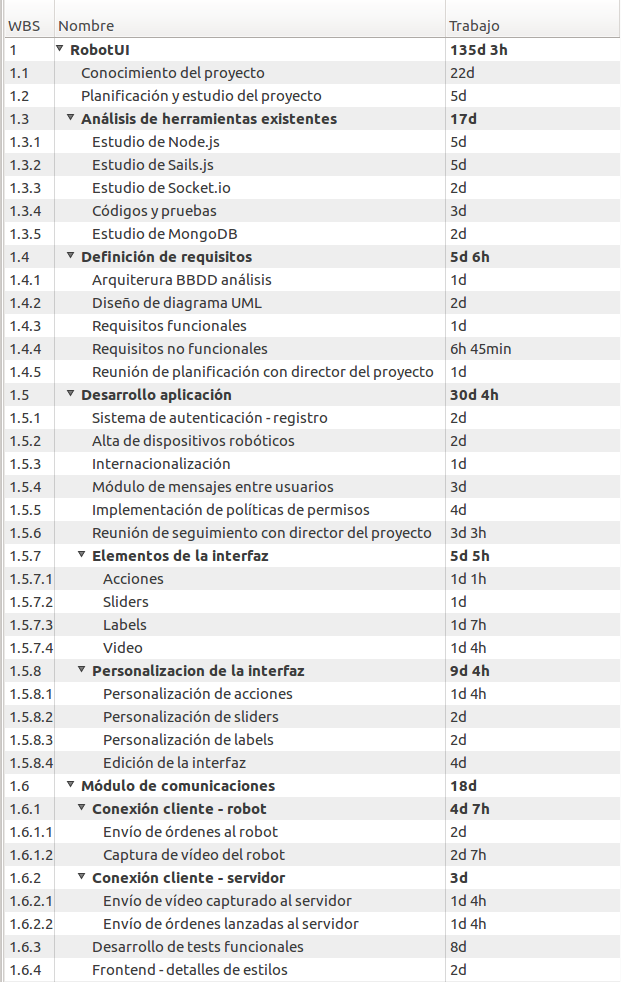
\includegraphics[scale=0.6]{imagenes/planificacion/descomposicion_tareas01.png}
  \end{center}
  \caption{Descomposición de las tareas implicadas en el desarrollo del proyecto (Primera Parte).}
  \label{gantt:tareas01}
\end{figure}


\begin{figure}
  \begin{center}
    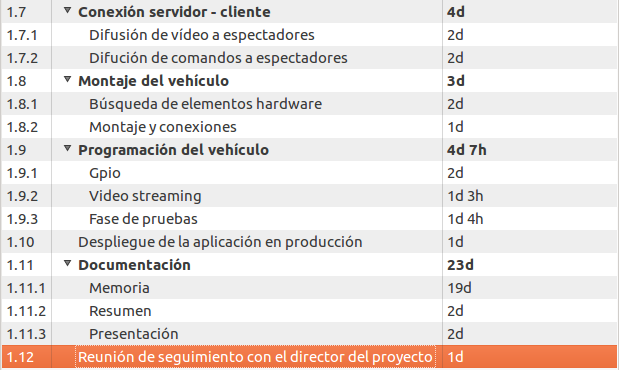
\includegraphics[scale=0.6]{imagenes/planificacion/descomposicion_tareas02.png}
  \end{center}
  \caption{Descomposición de las tareas implicadas en el desarrollo del proyecto (Segunda parte).}
  \label{gantt:tareas02}
\end{figure}

Los puntos más importantes del proyecto se han dividido en hitos, así como entregas que se definieron en cada reunión que se realizaba con el director del proyecto. 
También se ha definido una planificación temporal del desarrollo del proyecto mediante un diagrama de Gantt con la duración de las tareas recogidas en el panel de actividades de Trello.\\
\newpage


\section{Planificación temporal de tareas}

A continuación se definirán los diferentes hitos que componen el diagrama de Gantt divididos en las diferentes subtareas principales de cada uno de ellos:\\

\subsection{Hito 1: Planificación y análisis }
\label{subsec:hito1}

En esta primera etapa de desarrollo del proyecto final de carrera se realizaron los estudios previos necesarios para abordar cualquier proyecto de cierta envergadura.

Este hito se descompone en las siguientes tareas principales:

\begin{enumerate}
 \item Planificación y estudio del proyecto. En esta fase se centró en la elaboración de un documento, a modo borrador, con la idea a desarrollar, objetivos del proyecto y su alcance.
 \item Análisis de herramientas existentes, de las tecnologías a implementar, la arquitectura del sistema, las tecnologías de BD, visualización, para la selección de las herramientas más adecuadas 
 para afrontar el desarrollo con garantías y no sea necesaria una ``vuelta atrás'' por necesidad imperiosa de cambio de tecnología. En definitiva se buscaba una herramienta libre, con un respaldo de una comunidad importante
 y que resuelva la problemática o necesidad de trabajar con eventos en tiempo real.
\end{itemize}

\subsection{Hito 2: Definición de requisitos }
\label{subsec:hito2}

Este segundo hito queda dividido en las siguientes etapas:

\begin{enumerate}
 \item Elaboración de un documento formal con la propuesta de proyecto definiendo sus objetivos y alcance, para la aprobación por parte del director del proyecto.
 \item Se definen las clases del sistema, el modelo de la base de datos y la definición de requisitos funcionales y no funcionales. 
\end{enumerate}

\subsection{Hito 3: Comienzo de desarrollo de la aplicación}
\label{subsec:hito3}

En este tercer hito, uno de los de mayor magnitud, se comienza con el desarrollo de la aplicación, el cual queda dividido en las siguientes módulos.

\begin{enumerate}
 \item Implementación del módulo \emph{Usuario} con las funciones de registro, autenticación, configuraciones de idioma, entre otras.
 \item Implementación del módulo central de la aplicación \emph{Robot}
 \item Implementación del módulo de mensajes.
 \item Implementación del módulo de políticas de permisos.
\end{enumerate}


\subsection{ Hito 4: Desarrollo de la aplicación, módulo componentes }
\label{subsec:hito4}

En este hito, se trabaja en el desarrollo de los diferentes elementos que compondrán la interfaz de control. Tanto su parte de configuración y personalización. 
Cada elemento integrante de la interfaz lo denominamos componentes.\\

En definitiva, el hito queda dividido en el desarrollo de los siguientes componentes:

\begin{enumerate}
 \item \emph{Acciones}
 \item \emph{Sliders}
 \item \emph{Labels}
 \item \emph{Vídeo}
\end{enumerate}


\subsection{Hito 5: Desarrollo de la aplicación, módulo interfaz }
\label{subsec:hito5}

En este hito, se realiza la elaboración de la interfaz de control. Tanto su parte de configuración y personalización como la de visualización para su control. Este hito quedó dividido 
en las siguientes etapas:

\begin{enumerate}
 \item Impementación de la funcionalidad de configuración
 \item Implementación de la funcionalidad de control
\end{enumerate}


\subsection{Hito 6: Desarrollo del módulo de comunicaciones }
\label{subsec:hito6}

El presente hito, clasificado como crítico debido a su importancia. Debía realizar la integración de todos los módulos anteriores y dotarlos de la funcionalidad principal para la que han sido diseñados. Estar interconectados 
entre sí además de la elaboración de los test funcionales.

\begin{enumerate}
 \item Impementación de la conexión cliente - robot.
 \item Implementación de la conexión cliente - servidor.
 \item Desarrollo de test funcionales.
\end{enumerate}


\subsection{Hito 7: Construcción del vehículo de pruebas }
\label{subsec:hito6}

Se realiza la construcción y montaje e instalación software del vehículo de pruebas y comprobación de las diferentes conexiones.

\subsection{Hito 8: Programación del vehículo de pruebas }
\label{subsec:hito6}

Se realiza la programación del vehículo y se realizan pruebas de todo el conjunto junto con las correcciones necesarias.


\subsection{Hito 9: Documentación }
\label{subsec:hito6}

Se finaliza la memoria para la revisión por parte del director del proyecto y su posterior impresión. Se prepara la presentación para la defensa ante tribunal.


\section{Diagrama de Gantt}

A continuación se muestra el diagrama de Gantt donde quedan reflejados los diferentes hitos descritos en el punto anterior.

\begin{figure}
  \hspace*{.8in}{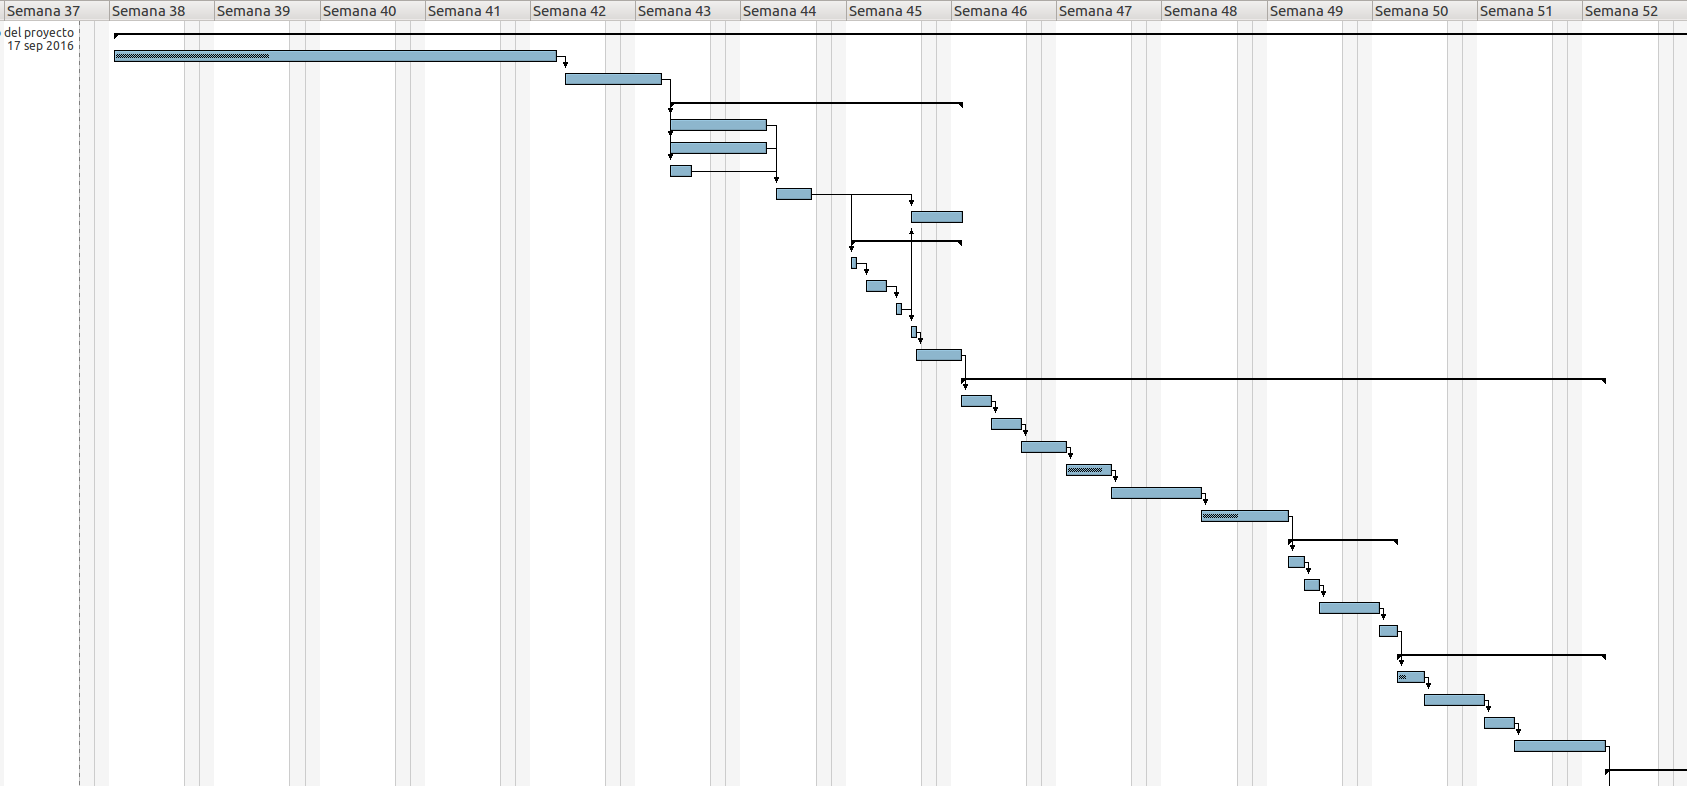
\includegraphics[scale=0.38,angle=270]{imagenes/planificacion/gantt01.png}}
  \caption{Diagrama de Gantt 1. Desarrollo del proyecto.}
\end{figure}

\begin{figure}
  \hspace*{.8in}{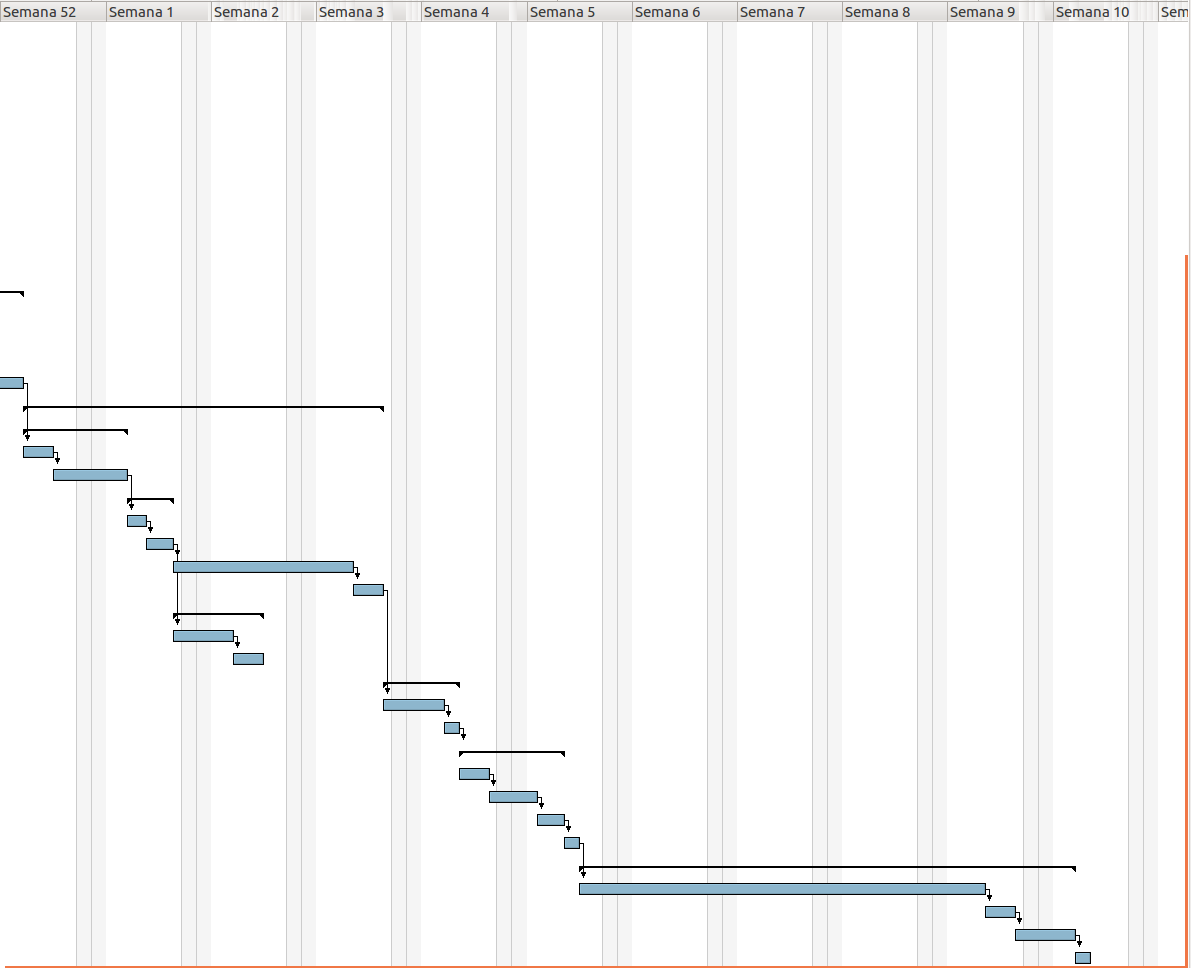
\includegraphics[scale=0.38,angle=270]{imagenes/planificacion/gantt02.png}}
  \caption{Diagrama de Gantt 2. Desarrollo del proyecto.}
\end{figure}